\documentclass[11pt]{article}

%Afegim els "packages" necessaris per generar el document
\usepackage[utf8]{inputenc}
\usepackage{graphicx}
\usepackage{fancyhdr}
\usepackage{hyperref}
\usepackage{tocloft}
\usepackage[T1]{fontenc}


\title{Instal·lació Allegro 5.1 (MAC)}
\author{Autor: Albert Lloveras Carbonell\\Revisió: Joaquim Porte Rodríguez}
\date{}

\renewcommand\contentsname{\huge Índex \vspace{8pt} \hrule}
\renewcommand{\cftsecleader}{\cftdotfill{\cftdotsep}}

%------------------------------------------------------------
%	Definició de Capçaleres i Peus de Pàgina
%------------------------------------------------------------

\fancypagestyle{pageStyle}{
	%Definim la capçalera de l'esquerra (Logo Salle)
	\fancyhead[L]{
		
\includegraphics[scale=0.25]{img/la_salle_logo.jpg}
	} 

	%Definim la capçalera de la dreta (Info Curs i Assignatura)
	\fancyhead[R]{
		\vtop{
			Manual d'instal·lació\\
			d'Allegro 5.1 + CodeLite (MAC)\\
		}
	}
	\fancyfoot[C]{} %Peu de pàgina central
	\fancyfoot[L]{Departament d'Enginyeria - Informàtica} %Peu de pàgina esquerra
	\fancyfoot[R]{\thepage} %Peu de pàgina dreta (Número de pàgina)	
	%Configuracions extra
	\renewcommand{\headrulewidth}{0pt} %Ocultem la línia de separació entre 		capçalera i bloc de text
	\renewcommand{\footrulewidth}{2pt} %Fixem la línia de separació entre peu de pàgina i bloc de text
	\setlength{\headheight}{67pt} %Fixem la mida de la capçalera	
	
}

%Definim la macro (nofooter) per poder amagar el peu de pàgina quan interessi
\fancypagestyle{nofooter}{
	\fancyfoot{}
	\renewcommand{\footrulewidth}{0pt}
}

%Definim la macro (nofooter) per poder amagar el peu de pàgina quan interessi
\fancypagestyle{empty}{
	\fancyfoot{}
	\fancyhead{}
	\renewcommand{\footrulewidth}{0pt}
	\renewcommand{\headrulewidth}{0pt}
}

\begin{document}

\pagestyle{empty}
\begin{center}

	%--- Logo de la portada --- %
	
\includegraphics[width=0.15\textwidth]{img/allegro.png}~\\[1cm]
	
	%---- Nom del programa --- %
	\textsc{\LARGE Allegro 5.1 + CodeLite}\\[1.5cm]
	
	%-- Nom del manual -- %
	\hrule
	\vspace{8pt}
	\huge{\bfseries Manual d'instal·lació (MAC)}
	\vspace{8pt}
	\hrule	
	\vspace{12pt	}

	% -- Nom de l'autor i del supervisor
	\noindent
	\begin{minipage}{0.4\textwidth}
		\begin{flushleft} \large
			\emph{Autor:}\\
			Albert \textsc{Lloveras}
		\end{flushleft}
	\end{minipage}%
	\begin{minipage}{0.4\textwidth}
		\begin{flushright} \large
			\emph{Revisió:} \\
			Joaquim \textsc{Porte}
		\end{flushright}
	\end{minipage}
	\vfill

\end{center}

%---- Índex ---- %
\newpage

\pagestyle{empty}
\tableofcontents


%---- Començament del document --- %
\newpage
\pagestyle{pageStyle}

\section{Introducció}
En aquest manual s'explicarà com realitzar la instal·lació de l'entorn de desenvolupament integrat (IDE) Code Lite juntament amb la llibreria gràfica Allegro5.1. La combinació d'aquests dos paquets de software ens permetran desenvolupar aplicacions de molt més gran envergadura que implementin interfícies gràfiques més potents que les interfícies de consola que hem estat utilitzant fins ara (línia de comandes).

\section{Obtenció del software necessari}
Abans de començar amb el procés ens farà falta descarregar el software que instal·larem al MAC. Per fer les coses fàcils, podeu trobar un comprimit amb tot allò que necessiteu al següent enllaç:

\begin{center}
	\url{http://goo.gl/QvPq1U}
\end{center}

\noindent Un cop completada la descàrrega, descomprimirem els continguts del \textit{.zip} a qualsevol carpeta del nostre ordinador. Al finalitzar la descompressió hauríem d'obtenir una carpeta amb el següents continguts:

\begin{center}
	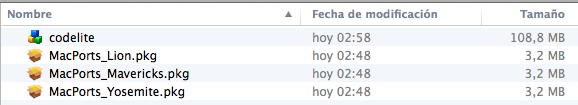
\includegraphics[scale=0.5]{img/Zip_Contents.png}
\end{center}

\noindent Per poder continuar amb la instal·lació de CodeLite i Allegro5.1 necessitarem instal·lar una utilitat anomenada \textit{MacPorts} que ens permetrà instal·lar de manera automàtica tot una sèrie de dependències de software i programes que necessita Allegro per funcionar. Per fer-ho, clicarem sobre un dels tres instal·ladors de \textit{MacPorts} que tenim a la carpeta on hem descomprimit els continguts del \textit{.zip}. \\

\noindent \textbf{Nota:} És important notar que haureu d'escollir l'instal·lador que porti al nom la versió del sistema operatiu de MAC que estigueu utilitzant al vostre ordinador.

\newpage
\noindent La finestra que s'hauria de mostrar al fer doble click sobre l'instal·lador de \textit{MacPorts} és la següent:

\begin{center}
	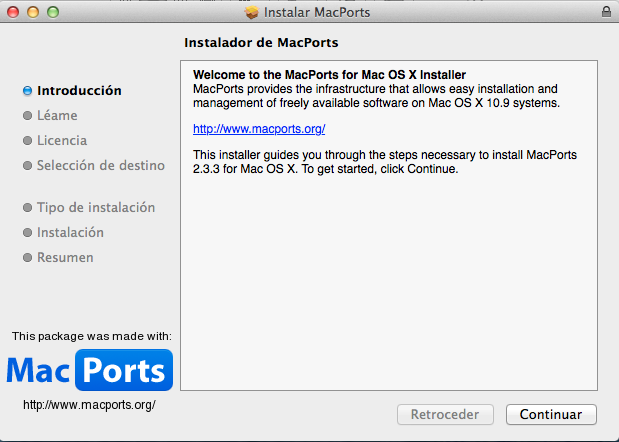
\includegraphics[scale=0.5]{img/MacPorts_Installation.png}
\end{center}

\noindent El procés d'instal·lació és molt senzill. Només cal anar prement el botó de \textit{Continuar} per anar avançant al llarg de l'instal·lador i, quan se'ns demani, acceptar la llicència del programa.\\

\noindent Finalment, hi haurà un moment que el botó \textit{Continuar} esdevindrà \textit{Instal·lar} i haurem de fer click a sobre d'aquest per començar la instal·lació.\\

\noindent \textbf{Nota:} És normal que quan comenci la instal·lació del programa se'ns demani que introduïm la clau d'administrador del sistema, ja que aquest programa haurà de tenir permisos d'administrador per poder, en un futur, instal·lar programes al nostre MAC des de línia de comandes.\\

\noindent Un cop finalitzada la instal·lació de \textit{MacPorts} podem prosseguir amb la instal·lació de CodeLite i d'Allegro5.1. No obstant això, \textbf{es recomana }realitzar un reiniciat de la màquina abans de continuar per tal d'assegurar que tot ha quedat perfectament instal·lat i integrat al sistema.


\newpage

\noindent Arribats a aquest punt, ja podem començar a instal·lar les dependències que necessita Allegro5.1. Per fer-ho, obrirem un terminal escrivint la paraula \textbf{terminal} al buscador spotlight. Per agilitzar el procés d'obertura del buscador, es pot emprar la següent combinació de tecles:

\begin{verbatim}
	                         CMD + ESPAI
\end{verbatim}

\noindent Si tot va bé, la finestra que ens hauria d'aparèixer hauria de ser la següent, en la que hi escriurem la següent comanda:

\begin{verbatim}
sudo port install zlib freetype jpeg libogg physfs libpng flac
libtheora +universal
\end{verbatim}

\begin{center}
	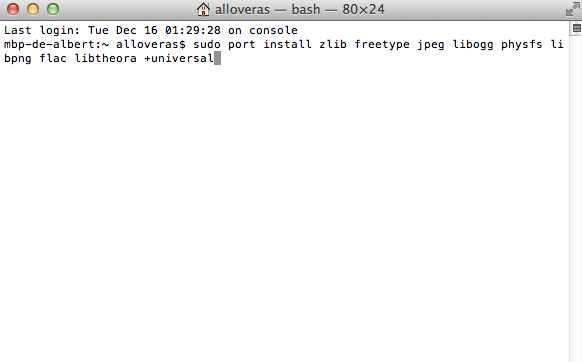
\includegraphics[scale=0.5]{img/Ports_Install_Libs.png}
\end{center}

\noindent \textbf{Nota:} És normal que al introduir la comanda anterior el programa torni a demanar la clau d'administador. El motiu d'això és que ens disposem a instal·lar nou software a l'ordinador i, per tant, li hem d'indicar que tenim permisos per fer-ho.

\newpage
\noindent Caldrà tenir una mica de paciència mentre s'instal·len les dependències ja que n'hi ha unes quantes. Un cop finalitzada la comanda anterior, llançarem la següent a través del mateix terminal tal i com es mostra a la següent imatge:

\begin{verbatim}
	sudo port install git cmake
\end{verbatim}

\begin{center}
	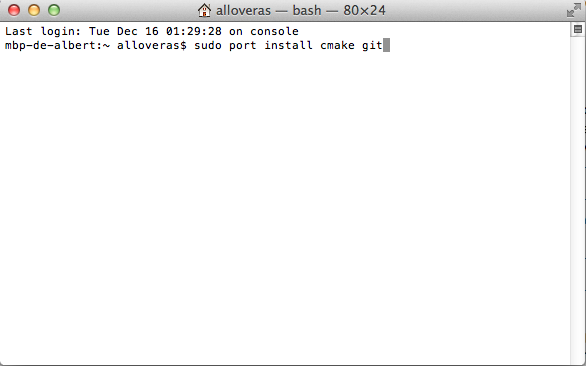
\includegraphics[scale=0.5]{img/Ports_Install_Git_Cmake.png}
\end{center}

\noindent Un cop finalitzada la instal·lació, ja estem llestos per començar la instal·lació d'Allegro 5.1. Per començar ens caldrà obtenir el codi font de la llibreria. Per descarregar-lo executarem la següent comanda al terminal tal i com es mostra a les imatges:

\begin{verbatim}
	git clone git://git.code.sf.net/p/alleg/allegro allegro
\end{verbatim}

\begin{center}
	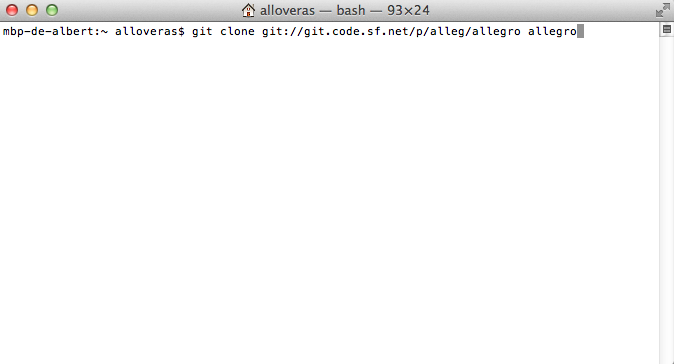
\includegraphics[scale=0.5]{img/Git_Clone.png}
\end{center}

\noindent La comanda anterior provocarà que se'ns cloni el codi font de la llibreria Allegro des del rebost públic d'Internet a una carpeta del nostre ordinador anomenada \textit{allegro}. Un cop completada la descàrrega, ens caldrà executar la següent comanda per entrar al directori on s'han descarregat les fonts:

\begin{verbatim}
	cd allegro
\end{verbatim}

\noindent Un cop dins del directori de les fonts d'Allegro executarem la comanda que configurarà Allegro per ser instal·lada al nostre ordinador. La comanda en concret és la següent:

\begin{verbatim}
	cmake CMakeLists.txt
\end{verbatim}

\begin{center}
	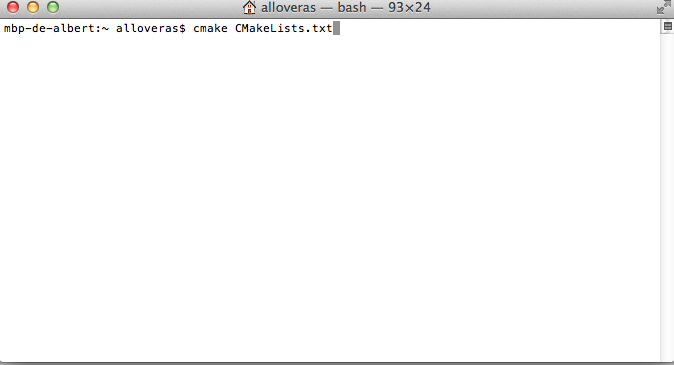
\includegraphics[scale=0.5]{img/Configure.png}
\end{center}

\noindent \textbf{Nota:} Aquest procés és normal que trigui una mica i que tregui bastantes línies de text per la pantalla. Caldrà ser pacients i esperar a que acabi.\\

\newpage
\noindent Un cop finalitzada la configuració, ja podrem començar a compilar la llibreria. Per fer-ho, caldrà executar la següent comanda tal i com mostrem tot seguit:

\begin{verbatim}
	make
\end{verbatim}

\begin{center}
		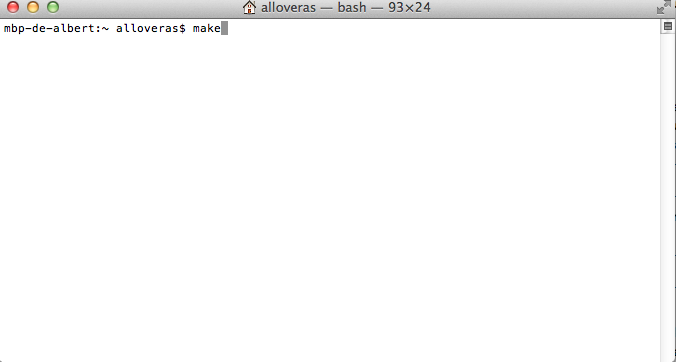
\includegraphics[scale=0.5]{img/Make.png}
\end{center}

\noindent \textbf{Nota:} Aquest procés també trigarà una estona i se'ns mostrarà per pantalla una sèrie de línies que indiquen el progrés de la compilació. Mentre compila poden aparèixer alguns \textit{warnings}. No obstant, no són perillosos i poden ser ignorats.\\

\noindent Ja per finalitzar, només quedarà moure els fitxers binaris que acabem de compilar a la carpeta del sistema que els hi correspon. Per fer-ho executarem al mateix terminal la següent comanda:

\begin{verbatim}
	sudo make install
\end{verbatim}

\noindent Un cop acabi la última comanda, ja tindrem instal·lada al nostre ordinador la llibreria Allegro5.1. Ara només ens quedarà instal·lar CodeLite per començar a desenvolupar.\\
 
\noindent Per instal·lar CodeLite, n'hi haurà prou en tornar a la carpeta on havíem descomprimit el \textit{.zip} que ens hem descarregat anteriorment i copiar el fitxer \textit{CodeLite} a la carpeta \textit{Aplicaciones} del MAC.

\newpage

\noindent A continuació es mostren unes imatges de com s'hauria de realitzar aquest procés:

\begin{center}
	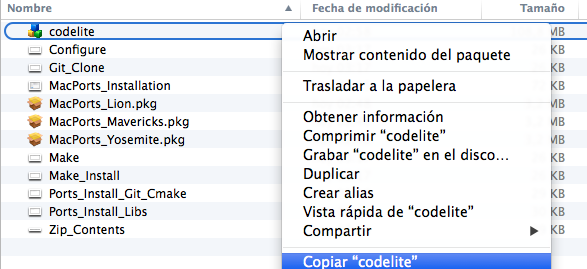
\includegraphics[scale=0.5]{img/Copiar_Code_Lite.png}\\\vspace{40px}
	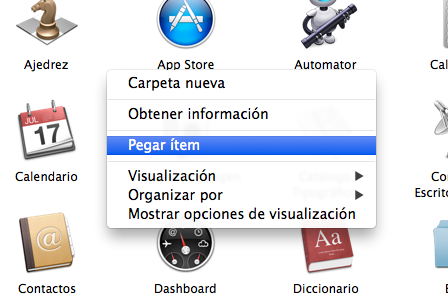
\includegraphics[scale=0.5]{img/Pegar_Aplicaciones.png}\\
\end{center}


\newpage

\section{Configuracions bàsiques de l'IDE}
\noindent Arribats a aquest punt, ja podrem obrir per primera vegada el CodeLite. Per fer-ho, farem click sobre el fitxer \textit{CodeLite} que acabem de copiar a la carpeta \textit{Aplicaciones} del MAC.\\

\noindent \textbf{Nota:} Pot ser que al intentar obrir \textit{CodeLite} us aparegui un missatge preguntant si realment desitgeu obrir el fitxer. Això es deu a que \textit{CodeLite} no és un programa desenvolupat per MAC ni cap companyia associada i, per tant, per defecte, el sistema operatiu en desconfia. No obstant, podeu fer click al botó \textit{Abrir} amb tota seguretat.\\

\noindent Si tot va bé i el programa s'inicia correctament, ens hauria d'aparèixer la finestra principal del programa juntament amb el següent missatge:

\begin{center}
	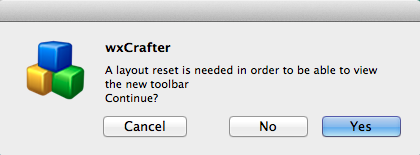
\includegraphics[scale=0.5]{img/Layout_Reset.png}
\end{center}

\noindent Per tal de que CodeLite s'adapti a al configuració de la nostre màquina és necessari que realitzem un reinicii del \textit{layout} dels menús de l'aplicació.\\\\
Per fer-ho, només cal que fem click al botó \textit{Yes} de la finestra emergent anterior.

\newpage

\noindent Tot seguit, després de reiniciar els menús ens apareixerà l'última finestra de configuració. Aquesta ens preguntarà sobre quin compilador volem que utilitzi CodeLite. El menú que ens apareixerà serà el següent:

\begin{center}
	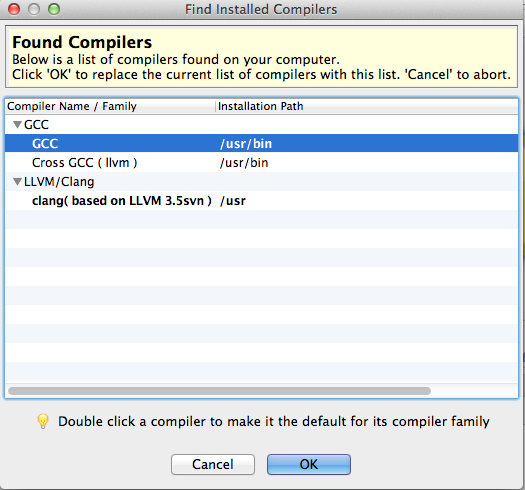
\includegraphics[scale=0.5]{img/Compiler_Selection.png}
\end{center}

\noindent Tal i com es veu a la imatge seleccionarem \textit{GCC} i farem click al botó \textit{OK}.\\


\noindent \textbf{Nota:} És molt important que no us equivoqueu al seleccionar el compilador, ja que sinó no podreu treballar amb Allegro, ja que la llibreria només s'ha instal·lat pel compilador GCC de la vostre màquina i no pas per la resta de compiladors que poguéssiu tenir instal·lats.\\

\noindent Fet tot això, ja tenim l'entorn de treball preparat. Ara només cal descarregar el projecte base que trobareu a l'eStudy i començar a treballar amb la pràctica.

\end{document}

